\documentclass{article}

% Language setting
% Replace `english' with e.g. `spanish' to change the document language
\usepackage[spanish]{babel}

% Set page size and margins
% Replace `letterpaper' with `a4paper' for UK/EU standard size
\usepackage[letterpaper,top=2cm,bottom=2cm,left=3cm,right=3cm,marginparwidth=1.75cm]{geometry}

% Useful packages
\usepackage{amsmath}
\usepackage{graphicx}
\usepackage{enumitem}
\usepackage{comment}
\usepackage{wrapfig}
\usepackage[colorlinks=true, allcolors=blue]{hyperref}

\title{AED Tema 5. Árboles equilibrados B y B+}
\author{Martín González Dios
\href{https://github.com/martindios}{\includegraphics[height=0.5cm]{github.png}}}


\begin{document}
\maketitle

Si queremos almacenar una cantidad muy grande de datos, podemos llegar al caso de que ocupe
varios bloques de disco, lo que supone tener que hacer varios accesos, ralentizando mucho el
tiempo de búsqueda. Para minimizar el problema del tiempo de acceso al disco (u otros medios
externos), se desarrollaron los \textbf{árboles B y árboles B+}.

\begin{wrapfigure}[]{r}{0.5\linewidth}
    \centering
    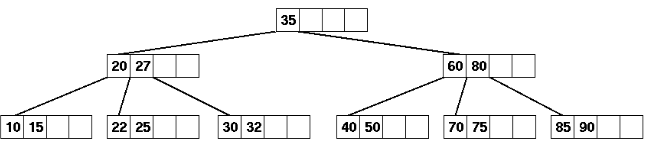
\includegraphics[width=\linewidth]{img-t5/img_357_90.png}
    \caption{Representación de árbol B}
\end{wrapfigure}

\section{Árboles B}
Arboles siempre equilibrados que minimizan el tiempo de búsqueda y borrado de elementos. En ellos, los nodos se agrupan en \textbf{páginas} (unidad a la que se accede en bloque, almacena la info. de un grupo de nodos identificados por claves). En un árbol B de \textbf{orden m} todas las páginas internas tienen entre $\lceil$m/2$\rceil$ y m ramas no vacías, y la raíz tiene 0 (si es la única página) o entre 2 y m ramas. En cada página interna hay (ramas - 1) claves, las cuales dividen las claves de sus ramas como un árbol de búsqueda. Todas las páginas hoja se encuentran en el mismo nivel, por eso es un \textbf{árbol totalmente equilibrado}.\\

\subsection{Inserción}
Se busca la página correspondiente, descendiendo por el árbol hasta llegar a la página hoja adecuada. Al querer insertar en dicha hoja, se pueden dar 2 casos:
\begin{itemize}
    \item Si la página no está llena, se inserta el elemento.
    \item Si la página está llena, ésta se divide en 2 (insertando ya el elemento en su sitio correspondiente) y el elemento mediana (el que ocupe la posición del medio) asciende en el árbol al nivel superiro, insertándose en la página padre, y de dicho elemento saldrán dos ramas, una a cada página generada en el elemento inferior (eliminándose, evidentemente, la rama que apuntaba a la página que se acaba de dividir, y que por tanto dejó de existir).
\end{itemize}

\subsection{Búsqueda}
Para buscar una clave en el árbol B se necesita partir de la página raíz y, evidentemente,
especificar la clave a buscar. Por tanto, estos serán los dos parámetros que se le pasen a la
función Buscar(). Se necesita un procedimiento auxiliar llamado Buscarnodo() que examina
para cada página dada si la clave se encuentra en ella o, en caso contrario, entre que dos claves
iría. En el segundo de los casos, se desciende a la página correspondiente del nivel inferior por
la rama que se encuentra entre los elementos, y se repite la búsqueda.

\newpage

\subsection{Eliminación}
En las eliminaciones también se pueden dar varios casos:
\begin{itemize}
    \item \textbf{La página donde se va a eliminar tiene más elementos que el mínimo}: si es una página hoja, se elimina sin problema. Si no es hoja, se sustituye el elemento por el predecesor en la hoja que salga de su rama derecha, y se elimina el elemento ahora en la página hoja.

    \item \textbf{La página donde se va a eliminar tiene el número mínimo de elementos}: se pueden dar 2 casos:
        \begin{itemize}
            \item Si una de las hojas hermanas tiene más elementos que el mínimo, se toma el elemento del extremo de dicha página, se sube a la padre, y de la padre se baja el correspondiente a la página en la que queremos hacer la eliminación, para tener más elementos que el mínimo y poder hacer la eliminación simple.

            \item Si todas las páginas hermanas tienen el mínimo de elementos, se unifican las dos páginas y se trae la mediana de ambas que está en la página padre. De esta forma la página padre reduce en uno sus elementos, y también en una de sus ramas.
        \end{itemize}
\end{itemize}

\section{Árboles B*}
\textbf{Optimización de los árboles B}. En la inserción, si la página está llena, se mueven elementos a una página hermana, posponiendo la división hasta que los hermanos estén completos. Con esto se reducen el número de divisiones.

\section{Árboles B+}

\begin{wrapfigure}[]{r}{0.5\linewidth}
    \centering
    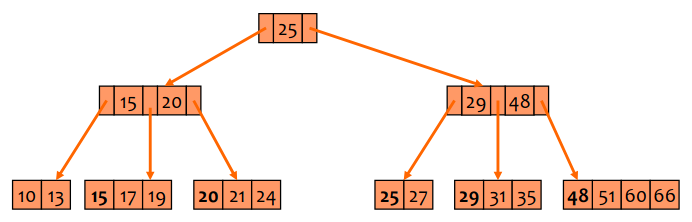
\includegraphics[width=\linewidth]{img-t5/img_683_70.png}
    \caption{Representación de árbol B+}
\end{wrapfigure}

Optimización de los árboles B para conseguir un recorrido secuencial más rápido.
Todos los elementos se encuentran en páginas hoja, de forma que algunos de estos elementos
aparecen duplicados en las páginas de niveles superiores únicamente con la función de actuar
como índices. Debido a esto, ocupan algo más de espacio en memoria, pero para árboles que se
modifican frecuentemente supone también un aspecto positivo, ya que evita la reorganización
del árbol, que era la operación más costosa en los árboles B.

\subsection{Inserción}
Por lo general es similar a la inserción en los árboles B, salvo por el caso en el que la página esté llena. En estos casos, el elemento mediana sube a la página padre. Pero también se mantiene en la página de la derecha resultante de la división en 2 de la página hoja original.

\subsection{Eliminación}
La eliminación es mucho más simple que en árboles B, ya que los elementos siempre están en
las páginas hojas. Se pueden dar dos casos:
\begin{itemize}
    \item Si tras eliminar el elemento la página todavía tiene el mínimo de elementos o más, no hay que hacer ninguna modificación.
    \item Si tras eliminar el elemento la página queda con menos elementos que el mínimo, hay redistribuir los elementos, borrando además un índice en la página de nivel superior, o cambiándolo.
\end{itemize}

\end{document}
